\chapter{نتیجه گیری}
این روش برای به دست ‌آوردن تصاویر کم حجم مفید است، اما  نتیجه آن از دید انسانی مناسب نیست.
روش‌های دیگری که تمرکز روی نزدیکی نتایج از دید انسان دارند مانند روشی که برای کاهش حجم
\lr{jpg}
استفاده می‌شود
به مراتب نتایج بهتری نسبت به این روش ارائه می‌دهند.

\section{استفاده‌های دیگر}
با این ایده‌های ابتدایی،‌می‌‌توان کاربرد‌های پیچیده‌تری از
\lr{SVD}
نیز پباده سازی کرد.

\subsection{حذف نویز}

به عنوان مثال،‌فرض کنید یک تصویر داریم که مقداری نویز دارد.
با روشی مشابه و درنظر گرفتن
$k$
مقدار اولیه مهم، می‌توان یک تقریب از تصویر به دست آورد که نویز آن تا حد خوبی کم شده
\cite{7067415}
.
البته این ساده ترین راه برای
\lr{denoising}
با
\lr{SVD}
می‌باشد و راه ‌های بهتری نیز داریم
\cite{10.1007/978-3-030-32456-8_43}
.


\begin{latin}
  \begin{python}
import numpy as np
import matplotlib.pyplot as plt
from PIL import Image

def image_to_matrix(image_path):
    img = Image.open(image_path)
    img_array = np.array(img)
    return img_array

def matrix_to_image(matrix, output_path):
    img = Image.fromarray(matrix)
    img.save(output_path)

def add_noise(image_array, noise_std=30):
    noise = np.random.normal(scale=noise_std, size=image_array.shape).astype(np.uint8)
    noisy_image = np.clip(image_array + noise, 0, 255).astype(np.uint8)
    return noisy_image

def denoise_image_svd(image_array, rank=None):
    # Apply SVD separately to each channel
    denoised_channels = []
    for channel in range(image_array.shape[2]):  # Iterate over channels (e.g., R, G, B)
        U, S, Vt = np.linalg.svd(image_array[:, :, channel], full_matrices=False)

        # Apply rank approximation
        if rank is not None:
            U = U[:, :rank]
            S = np.diag(S[:rank])
            Vt = Vt[:rank, :]

        denoised_channel = np.dot(U, np.dot(S, Vt))
        denoised_channel = np.clip(denoised_channel, 0, 255).astype(np.uint8)
        denoised_channels.append(denoised_channel)

    # Combine denoised channels into an RGB image
    denoised_image = np.stack(denoised_channels, axis=2)
    return denoised_image

# Example usage
if __name__ == '__main__':
    # Load an example image
    image_path = 'cat.png'
    original_image = image_to_matrix(image_path)

    # Add Gaussian noise to the image
    noisy_image = add_noise(original_image, noise_std=30)

    # Denoise the noisy image using SVD
    denoised_image = denoise_image_svd(noisy_image, rank=200)

    # Display and save results
    plt.figure(figsize=(10, 6))
    plt.subplot(1, 3, 1)
    plt.imshow(original_image)
    plt.title('Original Image')
    plt.axis('off')

    plt.subplot(1, 3, 2)
    plt.imshow(noisy_image)
    plt.title('Noisy Image')
    plt.axis('off')

    plt.subplot(1, 3, 3)
    plt.imshow(denoised_image)
    plt.title('Denoised Image (SVD, Rank=50)')
    plt.axis('off')

    plt.tight_layout()
    plt.show()

  \end{python}
\end{latin}

\begin{figure}
  \centering
  \resizebox{\textwidth}{!}{% Resize the figure to fit text width
    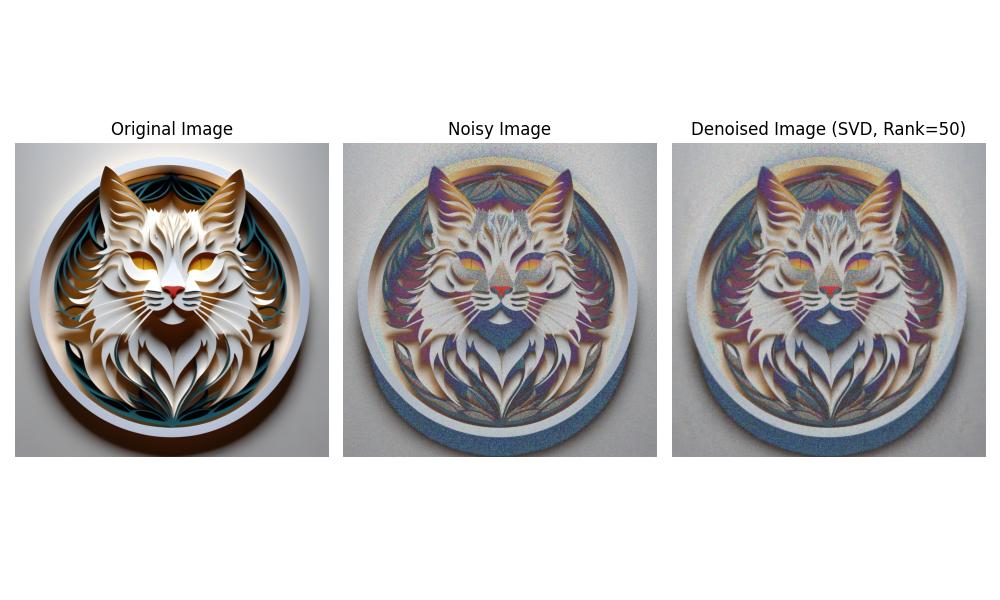
\includegraphics[width=\linewidth]{../output/denoise.jpg}
  }%
  \caption{\lr{Denoising}}
  \label{fig:img-denoise}
\end{figure}

\subsection{تشخیص چهره}
یکی دیگر از کاربرد‌های
\lr{SVD}
مقایسه تصاویر با مقایسه مقادیر اولیه آنهاست
\cite{TAI20161}
.
همچنین این مقادیر اولیه می‌توانند نقطه‌ی شروع برای یک الگوریتم یادگیری باشند
\cite{5539989}
.
a
